\chapter{\LaTeX}


The \LaTeX macro package contains a rich set of
predefined styles and format for technical documents based on
the \TeX typesetting engine\cite{oetiker1995not}. 

\chapter{Divergence theorem}

This chapter is taken from \url{http://en.wikipedia.org/wiki/Divergence_theorem}.

In vector calculus, the divergence theorem, also known as Gauss's theorem or
Ostrogradsky's theorem\cite{katz1979history}, is a result that relates the flow (that is, flux)
of a vector field through a surface to the behavior of the vector field inside the surface.

More precisely, the divergence theorem states that the outward flux of a vector
field through a closed surface is equal to the volume integral of the divergence
over the region inside the surface. Intuitively, it states that the sum of all
sources minus the sum of all sinks gives the net flow out of a region.

The divergence theorem is an important result for the mathematics of engineering,
in particular in electrostatics and fluid dynamics.

In physics and engineering, the divergence theorem is usually applied in three dimensions.
However, it generalizes to any number of dimensions. 
In one dimension, it is equivalent to the fundamental theorem of calculus.
In two dimensions, it is equivalent to Green's theorem.

The theorem is a special case of the more general Stokes' theorem.


\section{Intuition} \index{intuition}
If a fluid is flowing in some area, and we wish to know how much fluid flows
out of a certain region within that area, then we need to add up the sources 
inside the region and subtract the sinks. The fluid flow is represented by a
vector field, and the vector field's divergence at a given point describes 
the strength of the source or sink there. So, integrating the field's divergence
 over the interior of the region should equal the integral of the vector field 
over the region's boundary. The divergence theorem says that this is true.

\begin{figure}[htbp]
\centering
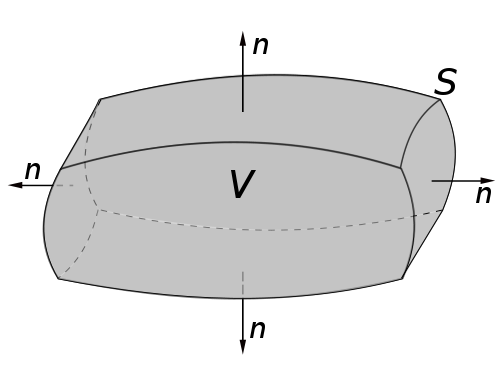
\includegraphics[width=0.5\textwidth]{Divergence_theorem.png} 
\caption{\label{fig:div_theorem}%
A region $V$ bounded by the surface $S=\partial V$ with the surface normal $\mathbf{n}$.}
\end{figure}

The divergence theorem is thus a conservation law which states that the volume
total of all sinks and sources, that is the volume integral of the divergence,
is equal to the net flow across the volume's boundary.

\section{Mathematical statement}
Suppose $V$ is a subset of $R^n$ (in the case of $n = 3$, $V$ represents a volume 
in 3D space) which is compact and has a piecewise smooth boundary $S$ 
(also indicated with $\partial V=S$). 
If $F$ is a continuously differentiable vector field defined on a neighborhood of $V$,
then we have:

\begin{equation}
  \iiint_V(\mathbf{\nabla}\cdot\mathbf{F}) \diff V =
  \oiint_S(\mathbf{F}\cdot\mathbf{n})\,\diff S.
\end{equation}

The left side is a volume integral over the volume $V$,
the right side is the surface integral over the boundary of the volume $V$.
The closed manifold $\partial V$ is quite generally the boundary of $V$
oriented by outward-pointing normals, and $\mathbf{n}$ is the outward pointing 
unit normal field of the boundary $\partial V$. 
($\diff \mathbf{S}$ may be used as a shorthand for $\mathbf{n} \diff S$.)
By the symbol within the two integrals it is stressed once more that $\partial V$
is a closed surface.
In terms of the intuitive description above, the left-hand side of the 
equation represents the total of the sources in the volume $V$, 
and the right-hand side represents the total flow across the boundary $\partial V$.

\section{Example}

Suppose we wish to evaluate
\begin{equation}
  \oiint_S \mathbf{F}\cdot\mathbf{n} \, \diff S,
\end{equation}
where $S$ is the unit sphere defined by
\begin{equation}
   x^2+y^2+z^2=1
\end{equation}
and $\mathbf{F}$ is the vector field
\begin{equation}
  \mathbf{F} = 2 x\mathbf{i} + y^2\mathbf{j} + z ^2\mathbf{k}.
\end{equation}

\appendix
\chapter{Math Typesetting Examples}

Math typeset examples goes here.
\begin{equation}
  - \frac{\rho}{\varepsilon} = \nabla\cdot \left(\nabla V\right) = \pDeriv[2]{V}{x} + \pDeriv[2]{V}{y} + \pDeriv[2]{V}{z}
\end{equation}

The speed of light in vacuum is approximately $\unit[3\times10^8]{m s^{-1}}$.

This is a test rule of length $1.2\,\mathrm{\mu m}$, $1.2\,\mathrm{μm}$, aka $\unit[1.2]{μm}$, aka \SI{1.2}{\micro\meter}.

\[
\begin{cases}
1 \\ 3 
\end{cases}
\]


